\begin{figure}[H]
    \centering
    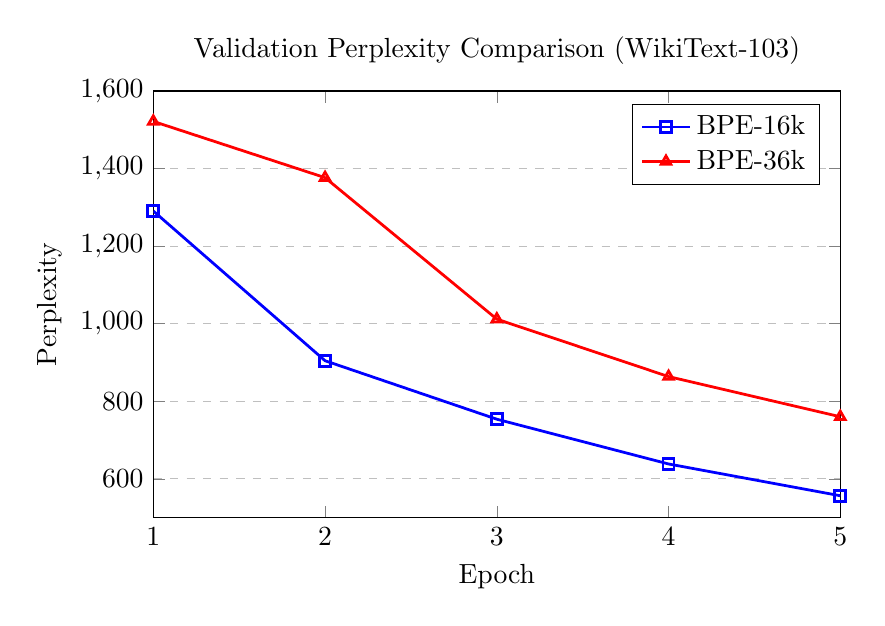
\begin{tikzpicture}
    \begin{axis}[
        title={Validation Perplexity Comparison (WikiText-103)},
        xlabel={Epoch},
        ylabel={Perplexity},
        xmin=1, xmax=5,
        ymin=500, ymax=1600,
        xtick={1,2,3,4,5},
        ytick={600, 800, 1000, 1200, 1400, 1600},
        legend pos=north east,
        ymajorgrids=true,
        grid style=dashed,
        width=0.85\textwidth,
        height=7cm,
    ]

    % K=16,000 Trend
    \addplot[
        color=blue,
        mark=square,
        line width=1pt,
        ]
        coordinates {
        (1, 1290.46)(2, 904.46)(3, 753.66)(4, 638.25)(5, 556.34)
        };
        \addlegendentry{BPE-16k}

    % K=36,000 Trend
    \addplot[
        color=red,
        mark=triangle,
        line width=1pt,
        ]
        coordinates {
        (1, 1521.50)(2, 1376.46)(3, 1011.68)(4, 863.56)(5, 759.99)
        };
        \addlegendentry{BPE-36k}

    \end{axis}
    \end{tikzpicture}
    \caption{Evolution of Validation Perplexity over 5 epochs for different vocabulary sizes.}
    \label{fig:ppl_k_comparison}
\end{figure}